\subsubsection{Base Controller}
\label{subsubsec:02psesTrajectory}
Das Fahrzeug wird von einem Knoten gesteuert, dessen Aufgabe darin besteht, die Stellgr"o"sen f"ur den Motor und die Lenkung zu berechnen und die verschiedenen Ziele f"ur den Rundkurs zu setzen.

\paragraph{Modelle}
Da die Lenkwinkel- und Geschwindigkeitsbefehle aus dem Navigation Stack in \si[per-mode=symbol]{\meter\per\second} und in \si[per-mode=symbol]{\radian} gepublished werden, m"ussen diese zu Stellgr"o"sen umgerechnet werden. Hierf"ur werden die im Abschnitt \ref{subsec:02modellbildung} beschriebenen Geschwindigkeits- und Lenkwinkelmodelle genutzt. Diese Stellgr"o"sen werden nach der Umrechnung als Topics f"ur die \texttt{uc\_bridge} gepublished.

\paragraph{Zielsetzung}
Damit eine Trajektorie geplant werden kann, muss dem Navigation Stack ein Ziel "ubergeben werden. Zum einen gibt es die M\"oglichkeit ein Ziel manuell in rviz vorzugeben und zum anderen ein Ziel in dem Topic \texttt{/move\_base\_simple/goal} zu ver\"offentlichen.\\
Um den Rundkurs zu fahren, wurden mehrere Ziele entlang der Strecke gesetzt, wie in Abbildung \ref{fig:goals} dargestellt. Mithilfe eines Z"ahlers wird jedes weitere Ziel aktiviert, sobald sich das Fahrzeug in einer Entfernung kleiner als 1,5m dazu befindet.

\begin{figure}[h]
	\centering
	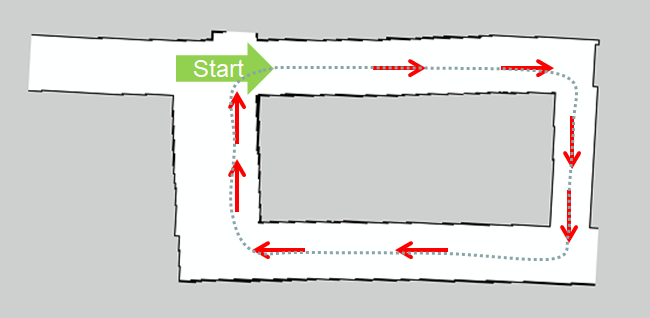
\includegraphics[width=0.8\textwidth,trim=2.4cm 0cm 0cm 1cm,clip]{pics/goals.png}
	\caption{Aufeinanderfolgenden Ziele entlang des Parcours}
	\label{fig:goals}
\end{figure}

\paragraph{Recovery Behavior}
Wie bereits im Kapitel \ref{subsubsec:02navigatinStack} erw"ahnt, kann es vorkommen, dass der lokale Planer aufgrund von Artefakten in der Costmap keine zul\"assige Trajektorie berechnen kann. Das Fahrzeug f"ahrt dann abwechselnd r"uck- und vorw"arts, ohne einen Ausweg zu finden. Um dieses Problem zu beheben, wurde ein eigenes \emph{Recovery Behavior} implementiert, welches dieses problematische Verhalten erkennen und das Obstacle Layer der Costmap leeren soll.\\
Diese Implementierung hat jedoch nicht funktioniert, da das richtige Layer beim Leeren der Costmap nicht gefunden werden konnte. Aus Zeitmangel konnte dieser Fehler nicht behoben werden.